
\subsection{Compiler(s), to the moon: beyond \texttt{-O3}}

Now that we have studied in-depth the behavior of the compiler given the default optimizations \texttt{-O}, we can further drive the compilation towards even more optimized code by giving even more specific flags to the compilers. 

For brevity, we define a set of these flags simultaneously to evaluate their cumulative impact on the kernel's performance, without explicitly define what is their separate impact on the generated assembly.

\begin{table}[H]
\centering
\begin{threeparttable}
\caption{Advanced compiler optimization flags and their expected effects.}
\label{tab:advanced_flags}
\begin{tabular}{lp{3cm}p{7cm}}
\toprule
\textbf{Flag} & \textbf{Category} & \textbf{Microarchitectural Effect} \\
\midrule
\texttt{-xHost} & Architecture & Instructs the compiler to target the highest instruction set available on the local host\tnote{1}, enabling the widest possible SIMD registers. \\
\midrule
\texttt{-fp-model fast=2} & Floating Point & Enables aggressive floating-point optimizations. It allows for reordering of operations and ignores strict IEEE 754 rules to maximize throughput\tnote{2}. \\
\midrule
\texttt{-fno-alias} & Memory & Asserts that no two pointers point to the same memory location, allowing the compiler to reorder loads and stores without "aliasing" checks. \\
\midrule
\texttt{-inline-level=2} & Inlining & Increases the intensity of function inlining to replace function calls with the actual function body, reducing branch penalties and call overhead. \\
\midrule
\texttt{-unroll-aggressive} & Loop Control & Enables aggressive loop unrolling heuristics, attempting to unroll loops even when the benefit is not immediately obvious to standard logic. \\
\midrule
\texttt{-unroll=4} & Loop Control & Specifically sets the unroll factor to 4, ensuring four iterations are processed as a single block to reduce loop-counter overhead. \\
\bottomrule
\end{tabular}

\begin{tablenotes}
    \footnotesize % This makes the font smaller
    \item[1] \textbf{AVX2} on the tested workstation, as reported in Table~\ref{tab:cpu_specs}.
    \item[2] For this reason, at test time the results of the kernel are explicitly checked to ensure results do not differ from the correct behavior.
\end{tablenotes}
\end{threeparttable}
\end{table}
\paragraph{Refactored Optimization Report.}
The following report summarizes the complex loop transformation strategy achieved with these aggressive flags.


The improvements with respect to the previous iteration are noticeable:

\begin{itemize}
    \item \textbf{Array Refs Replacement:} The compiler avoid the iterative request to obtain \texttt{C[i][j]} at each iteration, and decide to save its value in a register for a way-faster access.

    \item \textbf{Vectorization Width:} While standard \texttt{-O3} utilized a conservative vector length of 2 (128-bit), the addition of \texttt{-xHost} enables \textbf{vector length 4}.
    \item \textbf{Unroll and Jam:} The compiler now implements "Unroll and Jam" by a factor of 4. This technique unrolls the outer loops of a nest and fuses the resulting bodies, which significantly improves register reuse and ensure  a better use of the caches hierarchy\footnote{The exact steps implemented, along with the motivations, are explained in Appendix~\ref{subsec:unroll_jam}.}.
    \item \textbf{Vectorized Remainders:} The compiler now successfully \textbf{vectorizes the remainder loops}. This ensures that performance does not drop sharply at the boundaries of the matrix tiles.
\end{itemize}

\newpage
\begin{lstlisting}[style=CStyle, caption={Simplified ICC Report:\texttt{-O3 -xHost}.}]
LOOP BEGIN (i - tile )
    LOOP BEGIN (k - tile )
        LOOP BEGIN (j - tile )
            remark #25440: unrolled and jammed by 4 (pre-vector)    
            LOOP BEGIN (i - inner ) blocked by 128
                LOOP BEGIN (k - inner ) blocked by 128
                    LOOP BEGIN (j-vectorized) blocked by 128
                        remark #15289: vectorization support: unaligned access 
                        remark #15295: vectorization support: vector length 4
                        remark #15297: vectorization support: unroll factor set to 4
                        remark #15298: LOOP WAS VECTORIZED
                        remark #15300: Number of Array Refs Scalar Replaced In Loop
                    LOOP END
                    LOOP BEGIN (j-remainder)
                        remark #15301: REMAINDER LOOP WAS VECTORIZED
                        remark #15302: Number of Array Refs Scalar Replaced In Loop
                    LOOP END
                LOOP END
            LOOP END
        LOOP END
    LOOP END
LOOP END
\end{lstlisting}


\paragraph{Intel Advisor Roofline Analysis}

The impact of the \texttt{-xHost} flag is clearly visible in the transition to AVX2 execution. The kernel now achieves a computational throughput of \textbf{29.463 GFLOPS}. This is approximately double the performance of the standard \texttt{-O3} configuration, which reached 14.459 GFLOPS.

\begin{figure}[H]
\centering
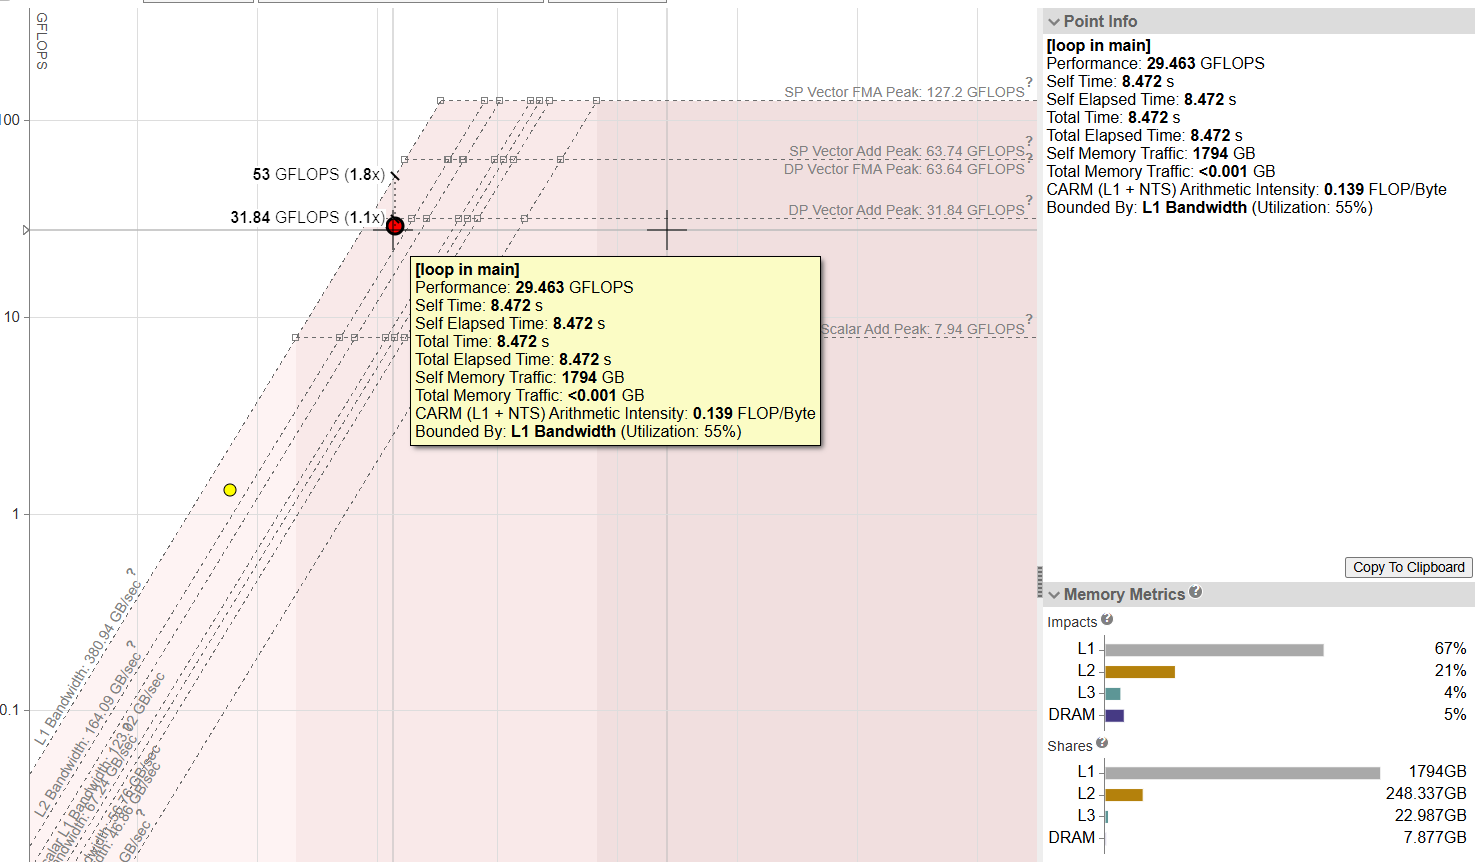
\includegraphics[width=1\textwidth]{Images/icc_better_roofline.png}
\caption{Roofline analysis for ICC \texttt{-O3 -Xhost etc...}.}
\label{fig:icc_better_roofline}
\end{figure}

The operational point on the Roofline model confirms this architectural shift, as the kernel now sits just under the DP Vector Add Peak (31.84 GFLOPS).

\paragraph{Performance comparison}

Lastly, we compare the performance of ICC against ICX\footnote{The ICX report indicates the same optimizations, with the exception that block sizes are $64 \times 64 \times 64$, whereas ICC utilizes $128 \times 128 \times 128$.} across a significantly broader domain of matrix sizes.

\begin{figure}[H]
\centering
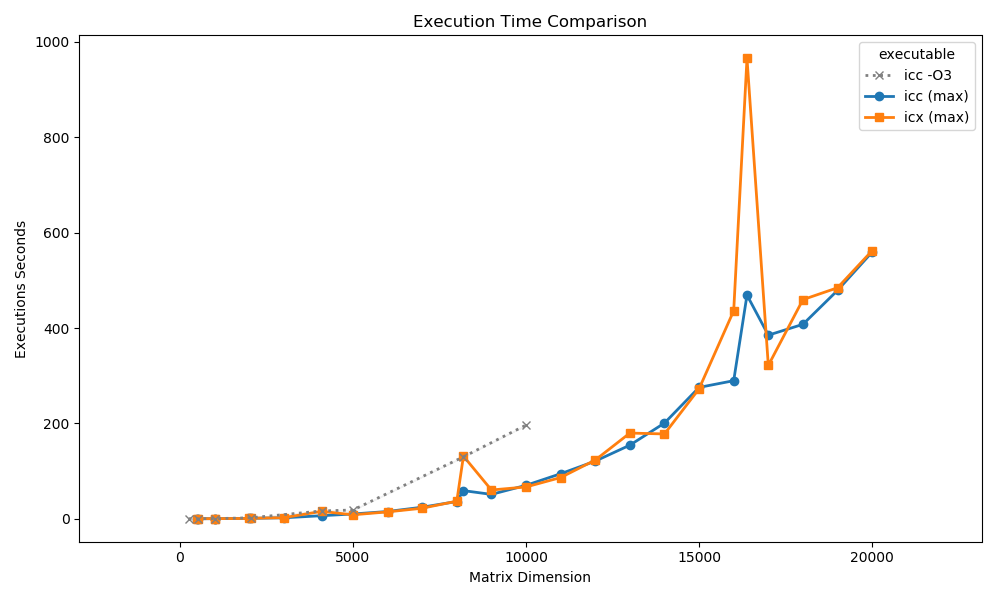
\includegraphics[width=0.8\textwidth]{Images/icc_icx_max.png}
\caption{Performance comparison of ICC and ICX with the advanced flags.}
\label{fig:icc_icx_better_comparison}
\end{figure}

It is immediately apparent that both highly optimized executables suffer a significant performance degradation when the matrix dimension $n$ is a power of 2 (e.g.,$n=4096$, $n=8192$, $n=16384$). 
In contrast, performance remains consistently high and scales more predictably when $n$ does not align with these boundaries.
This specific bottleneck is well motivated in the in-depth explanation in Appendix~\ref{subsec:caching}.

Nonetheless, we will also attempt once again to obtain another improvement: as noted in the optimization report, the main loop body still notify unaligned accesses, which limits the efficiency of the SIMD operations.

\subsubsection{A little price to pay for salvation? \texttt{-DALIGN}}
Note that a standard cache line is 64 bytes, which perfectly accommodates 8 double-precision (8-byte) values. 
When the matrix dimension $n$ (in particular the row's lenght) is not a multiple of 8, the compiler must generate "peeled" and "remainder" loops to handle those edge cases\footnote{Misalignment can also occur if the starting memory address is not aligned with the cache line boundary, but this is easily avoided by calling \texttt{posix\_memalign(ptr, 64, tot\_bytes)} at runtime.}.

By enabling the \texttt{-DALIGN} flag, we explicitly augment the matrix size from $n \times n$ to $n' \times n'$, where $n'$ is the smallest multiple of 8 greater than or equal to $n$.


The "overflow" cells in this padding area are initialized to zero to ensure they do not affect the mathematical results of the matrix multiplication (as explained in Appendix~\ref{subsec:padding}).

\paragraph{Practical Advantages.}

This approach, \textbf{while requiring slightly more memory}, provides several advantages:

\begin{itemize}
\item \textbf{Cache Line Alignment:} 
It is explicitly ensured by the code itself, without relying on the compiler's optimizations.

\item \textbf{Loop Simplification:} Because every row is now also a multiple of the register's capacity (4 doubles), the compiler no longer needs to generate auxiliary loops.

\item \textbf{SIMD Efficiency:} The hardware can perform 256-bit loads and stores at peak speed, as there is no longer a risk of a single vector instruction spanning across two different cache lines (nor incomplete register, that must be explicitly masked with zeros).
\end{itemize}


\paragraph{Compilation report}
The report produced by ICC clearly show a shortened, simplified version of the previous iteration\footnote{The  report from ICX showed once again how the only difference was in the choice of the block size, as before $64 \times 64 \times 64$.}.


\begin{lstlisting}[style=CStyle, caption={Optimization report of ICC with \texttt{-O3 -xHost -DALIGN}.}]
LOOP BEGIN (i-tile)
    LOOP BEGIN (k-tile)
        LOOP BEGIN (j-tile)
            remark #25440: unrolled and jammed by 4 (pre-vector)    
            LOOP BEGIN (i-inner) blocked by 125
                LOOP BEGIN (k-inner) blocked by 125
                    LOOP BEGIN (j-vectorized) blocked by 128
                        remark #15388: vectorization support: reference C[i][j] has aligned access
                        remark #15388: vectorization support: reference B[k][j] has aligned access
                        remark #15305: vectorization support: vector length 4
                        remark #15399: vectorization support: unroll factor set to 4
                        remark #15300: LOOP WAS VECTORIZED
                    LOOP END
                    LOOP BEGIN (j - remainder )
                        remark #15301: REMAINDER LOOP WAS VECTORIZED
                    LOOP END
                LOOP END
            LOOP END
        LOOP END
    LOOP END
LOOP END
\end{lstlisting}

\paragraph{Performance}

Figure~\ref{fig:icc_icx_aligned_comparison} demonstrates that even if \texttt{-DALIGN} successfully lowers execution times, matrices with dimensions power-of-two (and neighboring values) remain a major bottleneck.

\begin{figure}[H]
\centering
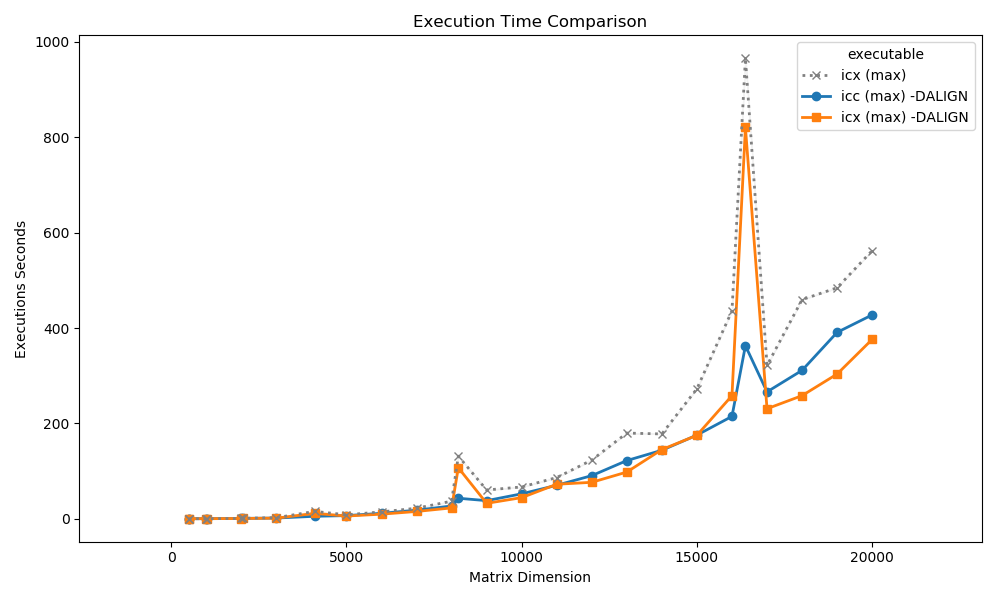
\includegraphics[width=0.8\textwidth]{Images/icc_icx_aligned.png}
\caption{Performance comparison of ICC and ICX with the advanced flags and -DALIGN.}
\label{fig:icc_icx_aligned_comparison}
\end{figure}

ICX achieves the best overall performance in standard cases but suffers the most extreme penalties at problematic dimensions. In contrast, ICC is slightly slower on average but far more stable, handling worst-case scenarios with much greater consistency.

Now we are equipped to  better understand the problem with those last implementations.
